\documentclass{article}
\usepackage{tikz}
\usepackage{geometry}
\usepackage[dvipsnames]{xcolor}
\pagestyle{empty}
\usepackage{luatexja}

\renewcommand{\kanjifamilydefault}{\gtdefault}
\renewcommand{\familydefault}{\sfdefault}
\newcommand{\docpaperwidth}{12.8cm}
\newcommand{\docpaperheight}{9.6cm}

\geometry{
  papersize={\docpaperwidth,\docpaperheight},
  margin=0.5cm,
  ignoreall=true
}

\usetikzlibrary{backgrounds}
\usetikzlibrary{calc}


\setlength{\parindent}{0cm}

% grid cell width
\newcommand{\grdclw}{1cm}
% grid cell half width
\newcommand{\grdclwh}{0.5cm}
% grid cell quater width 
\newcommand{\grdclwq}{0.25cm}

% grid cell height
\newcommand{\grdclh}{0.5cm}
% grid cell half height
\newcommand{\grdclhh}{0.25cm}

% grid cell quater height
\newcommand{\grdclhq}{0.125cm}

%baseline offset from center for horizontal text
\newcommand{\bsloffseth}{-0.1cm}

%baseline offset from cenete for vertical text
\newcommand{\bsloffsetv}{0.1cm} 

% grid column x position a
\newcommand{\grdclxa}{0.2cm}
% grid column x position b
\newcommand{\grdclxb}{\grdclxa + \grdclw}
% grid column x position c
\newcommand{\grdclxc}{\grdclxb + \grdclw}
% grid column x position d
\newcommand{\grdclxd}{\grdclxc + \grdclw}
% grid column x position e
\newcommand{\grdclxe}{\grdclxd + \grdclw}
% grid column x position f 
\newcommand{\grdclxf}{\grdclxe + \grdclw}
% grid column x position g
\newcommand{\grdclxg}{\grdclxf + \grdclw}
% grid column x position h
\newcommand{\grdclxh}{\grdclxg + \grdclw}

% grid column y position aa
\newcommand{\grdclya}{0.2cm}
% grid column y position ba
\newcommand{\grdclyb}{\grdclya + \grdclh}
% grid column y position ca
\newcommand{\grdclyc}{\grdclyb + \grdclh}
% grid column y position da
\newcommand{\grdclyd}{\grdclyc + \grdclh}

% grid left offset
\newcommand{\grdosl}{0.03cm}

% grid right offset
\newcommand{\grdosr}{-0.03cm}

% grid bottom offset
\newcommand{\grdosb}{0.03cm}

% grid top offset
\newcommand{\grdost}{-0.03cm}


\begin{document}
  \center
  % no hardware - software
  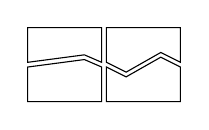
\begin{tikzpicture}[font=\tiny]

    \path [save path=\aacell]
      (\grdclxa + \grdosl, \grdclyb + \grdost)
      -- (\grdclxa + \grdosl, \grdclya + \grdosb) 
      -- (\grdclxb + \grdosr, \grdclya + \grdosb)
      -- (\grdclxb + \grdosr, \grdclyb + \grdost)
      -- ++(- \grdclwq - \grdosr, \grdclhq + \grdost)  
      -- cycle;

    \path [save path=\bacell]
      let \n1={3*\grdclwq} in
      (\grdclxa + \grdosl, \grdclyc + \grdost)
      -- (\grdclxa + \grdosl, \grdclyb + \grdosb)
      -- ++(\n1 - \grdosl, \grdclhq + \grdost)  
      -- (\grdclxb + \grdosr, \grdclyb + \grdosb)
      -- (\grdclxb + \grdosr, \grdclyc + \grdost)
      -- cycle;

    \path [save path=\abcell]
      (\grdclxb + \grdosl, \grdclyb + \grdost)
      -- (\grdclxb + \grdosl, \grdclya + \grdosb) 
      -- (\grdclxc + \grdosr, \grdclya + \grdosb)
      -- (\grdclxc + \grdosr, \grdclyb + \grdost)
      -- (\grdclxc + \grdosr - \grdclwq, \grdclyb + \grdost + \grdclhq)  
      -- (\grdclxb + \grdosl + \grdclwq, \grdclyb + \grdost - \grdclhq)  
      -- cycle;

    \path [save path=\bbcell]
      (\grdclxb + \grdosl, \grdclyc + \grdost)
      -- (\grdclxb + \grdosl, \grdclyb + \grdosb)
      -- (\grdclxb + \grdosl + \grdclwq, \grdclyb + \grdosb - \grdclhq)  
      -- (\grdclxc + \grdosr - \grdclwq, \grdclyb + \grdosb + \grdclhq)  
      -- (\grdclxc + \grdosr, \grdclyb + \grdosb)
      -- (\grdclxc + \grdosr, \grdclyc + \grdost)
      -- cycle;

    \draw [use path=\aacell];
    \draw [use path=\bacell];
    \draw [use path=\abcell];
    \draw [use path=\bbcell];


  \end{tikzpicture}
\end{document}

% vi: se ts=2 sw=2 et:

